\chapter{Order Finding}
\section{Introduction}

Now that we have discussed the phase estimation technique, it is time to apply it to an interesting computational problem: the \textbf{Order Finding} problem, which serves as a crucial step in the process of integer factoring. This forms the quantum core of \textbf{Shor's algorithm}; the remaining part of the algorithm is entirely classical and will be discussed in the next chapter.

We begin with a brief review of some foundational number-theoretic concepts, such as divisors, common divisors, and the greatest common divisor (GCD) of two integers.

The fast quantum algorithms for factoring and order finding are significant for at least three reasons:
\begin{enumerate}
    \item \textbf{Theoretical Importance:} They provide strong evidence that quantum computers may be inherently more powerful than classical computers, thus posing a credible challenge to the Strong Church-Turing Thesis.
    \item \textbf{Intrinsic Mathematical Value:} Both problems—factoring and order finding—are of intrinsic interest in number theory, and any efficient algorithm (quantum or classical) for these problems is valuable.
    \item \textbf{Practical Applications:} From a real-world perspective, efficient quantum algorithms for order finding and factoring can break widely used cryptographic protocols such as the RSA public-key cryptosystem.
\end{enumerate}

Of course, we know that factoring a number $x$ (a positive integer) means finding its non-trivial divisors—those integers other than $1$ and $x$ itself that divide $x$ exactly. If we are given two integers $x$ and $y$, then their \textit{common divisors} are the integers that divide both $x$ and $y$.

\begin{example}
For instance, consider the numbers $28$ and $42$. Their common divisors are:
\[
1, 2, 7, \text{ and } 14.
\]
Note that $4$ is not a common divisor, because although $4$ divides $28$, it does not divide $42$.
\end{example}


\begin{definition}
    \textbf{Greatest Common Divisor (GCD).} For two integers $x$ and $y$, their \emph{greatest common divisor} is the largest positive integer that divides both $x$ and $y$. This is commonly denoted as $\gcd(x, y)$.
\end{definition}

\noindent
For example, $\gcd(28, 42) = 14$, since $14$ is the largest integer that divides both $28$ and $42$. On the other hand, $\gcd(16, 21) = 1$, since there is no larger integer (other than $1$) that divides both $16$ and $21$.

\vspace{1em}

\begin{definition}
    \textbf{Relatively Prime.} Two integers $x$ and $y$ are said to be \emph{relatively prime} if $\gcd(x, y) = 1$. That is, they share no common divisors other than the trivial divisor $1$.
\end{definition}

\noindent
Note that two numbers can be relatively prime even if neither of them is a prime number. For example, $16$ and $21$ are both composite, but they are relatively prime because they have no common divisors other than $1$.

Superficially, the problem of finding common divisors resembles the problem of finding divisors (i.e., the factoring problem). If $x$ and $y$ are $n$-bit (binary) numbers, then a brute-force search for common divisors would involve checking among exponentially many possibilities as there are $O(2^n)$ possible numbers.

In fact, the problem of finding greatest common divisors is considerably easier than factoring. It has been known for a very long time that there is an efficient algorithm for computing GCDs. By ``very long time", we mean approximately 2300 years! That's when Euclid published his algorithm—now known as the \textit{Euclidean algorithm}. Of course, there were no computers back then, but Euclid's algorithm could be executed by hand and requires only $\mathcal{O}(n)$ arithmetic operations for $n$-digit numbers. This translates into a gate cost of $\mathcal{O}(n^2 \log n)$ on a modern computer. Let's remember Euclid's GCD algorithm, because we will make use of it later.

\vspace{1em}

Now, we briefly review a few more properties of numbers. Let $N \geq 2$ be an integer—not necessarily prime. Recall the set:
\[
\mathbb{Z}_N = \{0, 1, 2, \ldots, N - 1\}
\]
and define:
\[
\mathbb{Z}_N^* = \{x \in \mathbb{Z}_N \mid x \text{ has a multiplicative inverse mod } N\}
\]
The set $\mathbb{Z}_N^*$ forms a group under multiplication modulo $N$. For example:
\[
\mathbb{Z}_{21}^* = \{1, 2, 4, 5, 8, 10, 11, 13, 16, 17, 19, 20\}
\]
It turns out that $x$ has a multiplicative inverse modulo $N$ \textbf{if and only if} $\gcd(x, N) = 1$. For example, elements such as $3$, $6$, $7$, $12$, etc. (among others in $\mathbb{Z}_{21}$) are excluded from $\mathbb{Z}_{21}^*$ because they have nontrivial common divisors with $21$.

\begin{definition}
    (\textbf{Order of $a \in \mathbb{Z}_N^*$}) For any $a \in \mathbb{Z}_N^*$, define the order of $a$ modulo $N$ (denoted as $\operatorname{ord}_N(a)$) as the smallest positive integer $r$ such that
    \[
        a^r \equiv 1 \pmod{N}.
    \]
    This is the period of the sequence of powers of $a$ modulo $N$.
\end{definition}

The fact that such an $r$ always exists follows from Euler's theorem:

\begin{theorem}[Euler's Theorem]
    For any $a \in \mathbb{Z}_N^*$,
    \[
    a^{\varphi(N)} \equiv 1 \pmod{N}.
    \]
    where $\varphi(N)$ is Euler’s totient function, i.e., the number of integers less than $N$ that are relatively prime to $N$.
\end{theorem}

\begin{example}
    Show that the order of $x = 5$ modulo $N = 21$ is $6$.

    Let's take an element of $\mathbb{Z}_{21}^*$ and compute its powers. Suppose we pick $x = 5$. The powers of $5$ modulo $21$ are:
    \[
    5^0 \equiv 1,\quad 5^1 \equiv 5,\quad 5^2 \equiv 4,\quad 5^3 \equiv 20,\quad 5^4 \equiv 16,\quad 5^5 \equiv 17,\quad 5^6 \equiv 1 \pmod{21}.
    \]
    Notice that $5^6 \equiv 1 \pmod{21}$, and the sequence starts repeating after this. Hence, the order of $5$ modulo $21$ is $6$. Also note that $\varphi(21)=12$ and so, we can also see that $5^{12} \equiv 1 (\bmod 21)$.
\end{example}

\noindent
If we pick $x = 4$ instead of $5$, then the period is different. The powers of $4$ modulo $21$ are:
\[
4^0 \equiv 1,\quad 4^1 \equiv 4,\quad 4^2 \equiv 16,\quad 4^3 \equiv 1 \pmod{21},
\]
and so the period is $3$.

\medskip

\noindent
For positive integers $x$ and $N$, with $x < N$ and $\gcd(x, N) = 1$, the order of $x$ modulo $N$ is defined to be the smallest positive integer $r$ such that:
\[
x^r \equiv 1 \pmod{N}.
\]

\begin{example}
    Show that the order $r$ of $x$ modulo $N$ satisfies $r \leq N$.

    Since $\gcd(x, N) = 1$, Euler’s theorem tells us that
    \[
    x^{\varphi(N)} \equiv 1 \pmod{N},
    \]
    where $\varphi(N)$ is Euler’s totient function, i.e., the number of integers less than $N$ that are relatively prime to $N$. Since $\varphi(N) < N$, this guarantees that there exists some positive integer $r \leq \varphi(N) < N$ such that $x^r \equiv 1 \pmod{N}$.

    Therefore, $\operatorname{ord}_N(x) \leq \varphi(N) < N$.
\end{example}

Some additional notation will be helpful for discussing the Order Finding Problem. If $a$, $b$, and $N$ are integers with $N \geq 1$, we write
\[
a \equiv b \pmod{N}
\]
to mean that $N$ divides $a - b$, i.e., $N \mid (a - b)$.

As mentioned earlier, we let $\mathbb{Z}_N$ denote the set
\[
\mathbb{Z}_N = \{0, 1, 2, \ldots, N - 1\}.
\]
When equipped with addition and multiplication modulo $N$, this set forms a ring. If, in addition, $N$ is prime, then $\mathbb{Z}_N$ forms a finite field.

We also define the multiplicative group of integers modulo $N$, denoted by $\mathbb{Z}_N^*$:
\[
\mathbb{Z}_N^* = \{ a \in \mathbb{Z}_N \mid \gcd(a, N) = 1 \},
\]
which consists of all integers modulo $N$ that are relatively prime to $N$ (i.e., have a multiplicative inverse modulo $N$). The number of elements in $\mathbb{Z}_N^*$ is given by Euler’s totient function, denoted $\varphi(N)$. That is,
\[
\varphi(N) = |\mathbb{Z}_N^*|.
\]
When equipped with multiplication modulo $N$, the set $\mathbb{Z}_N^*$ forms an abelian group. This implies that for every element $a \in \mathbb{Z}_N^*$, there exists a unique inverse $b \in \mathbb{Z}_N^*$ such that
\[
ab \equiv 1 \pmod{N}.
\]
We denote this element by $a^{-1} \pmod{N}$, or simply $a^{-1}$ when the modulus is clear from context. We now define the central concept in the Order Finding problem.

Such an $r$ always exists from Euler's theorem. This guarantees that some power of $a$ must return to $1$, and so the order of $a$ is well-defined. Moreover, the order $\operatorname{ord}_N(a)$ always divides $\varphi(N)$, since the minimal such $r$ must divide any larger $k$ for which $a^k \equiv 1 \pmod{N}$.

Let $a = 4$ and $N = 35$. Since $\gcd(4, 35) = 1$, we have $4 \in \mathbb{Z}_{35}^*$.

Computing the powers of $4$ modulo $35$:
\[
\begin{aligned}
4^1 &\equiv 4 \pmod{35},\\
4^2 &\equiv 16 \pmod{35},\\
4^3 &\equiv 29 \pmod{35},\\
4^4 &\equiv 11 \pmod{35},\\
4^5 &\equiv 9 \pmod{35},\\
4^6 &\equiv 1 \pmod{35}.
\end{aligned}
\]
Hence, $\operatorname{ord}_{35}(4) = 6$.

\medskip

This notion of order is at the heart of the quantum part of Shor’s algorithm. The quantum subroutine efficiently finds this period $r = \operatorname{ord}_N(a)$, which enables the factoring of $N$ in the full algorithm.


Now that we know how the order of a given element $a \in \mathbb{Z}_N^*$ is defined, we can state the order finding problem.

\section{The Problem Definition}

\begin{definition}[Order Finding Problem]
\textbf{Input:} A positive integer $N \geq 2$ and an element $a \in \mathbb{Z}_N^*$. That is, $\gcd(a, N) = 1$. These are assumed to be $n$-bit (binary) integers.

\textbf{Output:} The order of $a$ modulo $N$, denoted $\operatorname{ord}_N(a)$, which is the smallest positive integer $r$ such that
\[
a^r \equiv 1 \pmod{N}.
\]
\end{definition}

\section{The Classical Solution}

Classically, the order-finding problem is believed to be hard. The most straightforward approach is to compute successive powers of $a$ modulo $N$—that is, compute $a, a^2, a^3, \dots$, until we find the smallest $r$ for which $a^r \equiv 1 \pmod{N}$. Unfortunately, this brute-force method can take exponential time in the number of bits $n = \lceil \log_2 N \rceil$, since the order $r$ can be as large as $\varphi(N)$, which itself can be exponential in $n$.

While each modular exponentiation can be performed efficiently using the method of repeated squaring (see Section~\ref{subsec:repeated_squaring_trick}), the sheer number of candidate exponents to check renders the overall brute-force solution exponential in $n$. To date, no known classical algorithm solves the order-finding problem in time polynomial in the number of bits required to specify the inputs.

Why, then, should we care about efficiently solving this problem? At first glance, it may appear to be an abstract question in number theory. However, it turns out that the factoring problem—a problem of profound importance in cryptography—reduces to the order-finding problem. That is, if we had an efficient algorithm (classical or quantum) for finding orders, then we could use it to efficiently factor large integers. We will see how factor finding reduces to order finding in the next chapter.

\section{The Quantum Solution}

Let us now describe a quantum algorithm for solving the order-finding problem. Given an input instance to the order-finding problem—namely, two $n$-bit numbers $N$ and $a$, where $a \in \mathbb{Z}_N^*$—the goal is to compute $r = \operatorname{ord}_N(a)$, the order of $a$ modulo $N$.

Our strategy is to reduce order-finding to the quantum phase estimation problem. To use phase estimation, we require two components: a unitary operator $U$ and an eigenvector of $U$. We will construct both based on modular arithmetic.

Assume $N \geq 2$ is given, and let $n = \lceil \log_2 N \rceil$ be the number of bits needed to encode elements of $\mathbb{Z}_N$ in binary. Given any $a \in \mathbb{Z}_N^*$, define the $n$-qubit transformation $M_a$ as:
\begin{equation}
M_a \ket{x} = \ket{a x \bmod N}
\label{eq:ord_find}
\end{equation}
for all $x \in \mathbb{Z}_N$. This definition covers inputs $0 \leq x < N$. For values $N \leq x < 2^n$, which lie outside of $\mathbb{Z}_N$, we define $M_a \ket{x} = \ket{x}$ to ensure a complete, well-defined unitary operator on the full $2^n$-dimensional space. Although these values will never be queried in our algorithm, this extension ensures that $M_a$ is defined on the entire Hilbert space. We now need to prove that the transformation defined in equation~\eqref{eq:ord_find} is unitary.

\subsection*{Proof of unitarity of $M_a$}
Let us show that $M_a$ is unitary. We can write the full operator $M_a$ acting on the $2^n$-dimensional Hilbert space as:
\[
M_a = \begin{pmatrix}
    \tilde{M}_a & 0 \\
    0 & I
\end{pmatrix}
\]
where $\tilde{M}_a$ is the submatrix acting on basis states $\ket{y}$ for $0 \leq y < N$, and $I$ is the identity acting on states $\ket{y}$ for $N \leq y < 2^n$.

It suffices to show that $\tilde{M}_a$ is unitary. Consider:
\[
\bra{y'} \tilde{M}_a^\dagger \tilde{M}_a \ket{y} = \braket{a y' \bmod N | a y \bmod N}
\]
Since $a \in \mathbb{Z}_N^*$ is invertible modulo $N$, we have that $a y' \equiv a y \pmod{N} \iff y' \equiv y \pmod{N}$ using properties of modular arithmetic since $a$ is co-prime (or relatively prime i.e. $\gcd(x,N)=1$) to $N$. Given that both $y$ and $y'$ lie in $\{0, \dots, N-1\}$, this implies $y = y'$. Hence,
\[
\bra{y'} \tilde{M}_a^\dagger \tilde{M}_a \ket{y} = \delta_{y, y'}
\]
and thus $\tilde{M}_a$ is unitary. Consequently, $M_a$ is unitary as well.

The transformation $M_a$ is reversible and hence unitary. This follows from the observation that multiplication by $a$ modulo $N$ defines a bijection on $\mathbb{Z}_N$, because $a$ has a multiplicative inverse modulo $N$ (since $\gcd(a, N) = 1$). Thus, $M_a$ has an inverse $M_{a^{-1}}$, and we have $M_{a^{-1}} M_a = I$.

This unitary transformation $M_a$ will serve as the basis for the quantum phase estimation subroutine used to find the order $r = \operatorname{ord}_N(a)$. In the next section, we will construct eigenstates of $M_a$ and apply phase estimation to extract the hidden period.

There are two important requirements for applying the phase estimation procedure: 

\begin{enumerate}
    \item We must have an efficient procedure to implement the controlled-$U^{2^j}$ operation for any integer $j$.
    \item We must be able to efficiently prepare an eigenstate $\ket{\psi}$ of $U$ with a non-trivial eigenvalue, or at least a superposition of such eigenstates.
\end{enumerate}

Let us now consider applying the transformation $M_a$ to the phase estimation procedure. It will turn out that doing so allows us to determine the order of $a$ modulo $N$. This motivates the need for two things in our quantum algorithm:
\begin{enumerate}
    \item An efficient implementation of the controlled-$M_a^{2^j}$ operations, i.e., the controlled modular exponentiation $\Lambda_m(M_a)$:
    \[
    \Lambda_m(M_a) \ket{k} \ket{x} = \ket{k} \ket{a^k x \bmod N}
    \]
    \item A means to prepare (or sample from a superposition of) the eigenvectors $\ket{\psi_j}$ of $M_a$.
\end{enumerate}
These ingredients, combined with quantum phase estimation, allow us to determine the order $r = \operatorname{ord}_N(a)$ with high probability.

\subsection{Multiplicity-Controlled \texorpdfstring{$M_a$}{Ma} Gate}
To apply the quantum phase estimation procedure to $M_a$, we must implement controlled applications of powers of $M_a$, specifically a controlled-$M_a^k$ operation. Fortunately, a reversible circuit implementing $M_a$ can be constructed efficiently, assuming that the functions
\[
f(y) = ay \bmod N \quad \text{and} \quad g(y) = a^{-1}y \bmod N
\]
are efficiently computable by Boolean circuits. These correspond to modular multiplication and modular inversion, which are known to admit efficient classical and quantum implementations.

In the context of phase estimation, the transformation we need takes the following form:
\[
\Lambda_m(M_a)\ket{x}\ket{y} = \ket{x}\ket{a^x y \bmod N}
\]
where $m$ is the number of control bits, i.e., the number of bits of precision required for phase estimation. This transformation is effectively a \textbf{modular exponentiation circuit}, controlled on a register of size $m$.

\paragraph{Gate Complexity.} Known techniques for modular exponentiation enable the efficient implementation of this operation. Specifically, the transformation $\Lambda_m(M_a)$ can be implemented using $\mathcal{O}(mn^2)$ quantum gates, where:
- $m$ is the number of bits of precision required in the phase estimation step.
- $n = \lceil \log_2 N \rceil$ is the number of bits needed to represent elements of $\mathbb{Z}_N$.

As we will see later, choosing $m = \mathcal{O}(n)$ is sufficient to recover the order $r = \operatorname{ord}_N(a)$ with high probability.

\paragraph{Circuit Structure.} This circuit essentially performs repeated squaring to compute $a^x \bmod N$ for a given control input $x \in \{0,1,\ldots,2^m - 1\}$. The entire sequence of controlled-$U^{2^j}$ operations required by the phase estimation routine can be realized using such multiplicity-controlled modular exponentiation.

Below is a sketch of the multiplicity-controlled $U_{a,N}$ gate:

\begin{figure}[ht]
    \centering
    \begin{quantikz}
        \lstick{$\ket{x}$} & \ctrl{1} & \rstick{$\ket{x}$} \\
        \lstick{$\ket{y}$} & \gate{U_{a,N}^x} & \rstick{$\ket{a^x y \bmod N}$}
    \end{quantikz}
    \caption{Multiplicity-controlled $U_{a,N}$ gate}
    \label{fig:multicontrlU}
\end{figure}

For each $x \in \{0,1\}^m \equiv \{0,1,\ldots,2^m - 1\}$ and $y \in \mathbb{Z}_N^*$, this gate maps the joint state $\ket{x}\ket{y}$ to:
\[
\ket{x}(U_{a,N})^x \ket{b} = \ket{x} \ket{a^x b \bmod N}
\]

\paragraph{Efficiency via Structure.} We can compute this efficiently (in terms of both $m$ and $n$) using the \textbf{repeated squaring trick}, which computes $a^x \bmod N$ using at most $\mathcal{O}(n \log n)$ gates per modular multiplication. Since we may need to repeat this for each of the $m$ control bits, the total complexity becomes $\mathcal{O}(mn \log n)$ gates for modular exponentiation, and $\mathcal{O}(mn^2)$ gates when full arithmetic costs are accounted.

\paragraph{Remark.} In general, the ability to efficiently compute a unitary $U$ does not imply that a multiplicity-controlled-$U$ operation can also be efficiently implemented. However, the unitary $U_{a,N}$ derived from modular multiplication enjoys special algebraic properties that allow for this efficient construction.

We will now see modular exponentiation performed using repeated squaring trick in detail.

\subsection*{Modular Exponentiation}

How can we compute the sequence of controlled-$U^{2^j}$ operations used by the phase estimation procedure as part of the order-finding algorithm? That is, we wish to compute the transformation:
\begin{align*}
    \ket{x}\ket{y} &\longrightarrow \ket{x} U^{x_{m-1} 2^{m-1}} \cdots U^{x_0 2^0} \ket{y} \\
    &= \ket{x} \ket{a^{x_{m-1} 2^{m-1}} \cdots a^{x_0 2^0} y \bmod N} \\
    &= \ket{x} \ket{a^{x_{m-1} 2^{m-1}} \cdots a^{x_0 2^0} y \bmod N}
\end{align*}

Thus, the sequence of controlled-$U^{2^j}$ operations used in phase estimation is equivalent to multiplying the contents of the second register by the modular exponential $a^x \bmod N$, where $x$ is the value in the control register. This transformation may be implemented efficiently using techniques from reversible computation.

\paragraph{Basic Strategy.} The basic idea is to:
\begin{enumerate}
    \item Reversibly compute the value $a^x \bmod N$ into a third ancillary register,
    \item Multiply the second register by $a^x \bmod N$,
    \item Use \emph{uncomputation} to erase the contents of the third register and restore it to zero.
\end{enumerate}

\paragraph{Stage 1: Precomputing Powers.}  
We begin by precomputing the powers $a^{2^j} \bmod N$ for $j = 0,1,\ldots,m-1$. This is done as follows:
\begin{itemize}
    \item Compute $a^2 \bmod N$ by squaring $a$ modulo $N$,
    \item Then compute $a^4 \bmod N$ by squaring $a^2 \bmod N$,
    \item Continue until $a^{2^{m-1}} \bmod N$ is computed.
\end{itemize}

Here, we will later see that $m = 2n + 1 + \left\lceil \log_2\left(2 + \frac{1}{2\epsilon} \right) \right\rceil = \mathcal{O}(n)$ suffices, so a total of $t-1 = \mathcal{O}(n)$ squaring operations are needed. Each squaring operation can be performed in $\mathcal{O}(n^2)$ gates using a standard long multiplication circuit, resulting in a total cost of:
\[
\mathcal{O}(n) \times \mathcal{O}(n^2) = \mathcal{O}(n^3)
\]
for the first stage.

\paragraph{Stage 2: Modular Exponentiation.}

The modular exponentiation $x^z \bmod N$ can be reconstructed from the identity:
\[
a^x \bmod N = a^{x_{m-1} 2^{m-1}} \cdots a^{x_0 2^0} \bmod N
\]
This implies that for every bit $x_j$ of the control register (with $j$ from $0$ to $m-1$), if $x_j = 1$, we multiply by $a^{2^j} \bmod N$. This gives a product of at most $m = \mathcal{O}(n)$ terms, each requiring a modular multiplication.

Each modular multiplication costs $\mathcal{O}(n^2)$ gates, so the total cost of computing $a^x \bmod N$ is again:
\[
\mathcal{O}(n) \times \mathcal{O}(n^2) = \mathcal{O}(n^3)
\]

\paragraph{Final Reversible Circuit.}  
Using the above two stages, we construct a reversible quantum circuit that takes a $m$-bit input register $\ket{x}$ and an $n$-bit input register $\ket{y}$ and computes the transformation:
\[
\ket{x}\ket{y} \longrightarrow \ket{z} \ket{a^x y \bmod N}
\]
The computation uses $\mathcal{O}(n^3)$ quantum gates. This circuit provides the necessary modular exponentiation component for performing the controlled unitary operations in phase estimation during order-finding.

\paragraph{Remark.}  
While $\mathcal{O}(n^3)$ is efficient enough for our purposes, more sophisticated multiplication algorithms (e.g., Karatsuba or Schönhage-Strassen methods) can reduce the asymptotic cost further. Nonetheless, this basic method provides an intuitive and practical foundation.

\subsection{How to construct \texorpdfstring{$\ket{\psi_j}$}{psij}?}

What are the eigenvectors and eigenvalues of $M_a$? It turns out that there are many, but we only need to consider a subset of them. Let $r$ be the order of $a \in \mathbb{Z}_N^*$, i.e., the smallest positive integer such that $a^r \equiv 1 \mod N$. Consider the vector:
\[
\ket{\psi_0} = \frac{1}{\sqrt{r}} \left( \ket{1} + \ket{a} + \ket{a^2} + \ldots + \ket{a^{r-1}} \right)
\]
(From this point on, all operations inside kets are assumed to be modulo $N$.)

To verify that $\ket{\psi_0}$ is indeed an eigenvector of $M_a$, we compute:
\begin{align*}
    M_a \ket{\psi_0} &= \frac{1}{\sqrt{r}} \left( \ket{a} + \ket{a^2} + \ket{a^3} + \ldots + \ket{a^r} \right) \\
    &= \frac{1}{\sqrt{r}} \left( \ket{a} + \ket{a^2} + \ldots + \ket{a^{r-1}} + \ket{1} \right) \\
    &= \ket{\psi_0}
\end{align*}
Hence, $\ket{\psi_0}$ is an eigenvector with eigenvalue $1$.

Here is another eigenvector:
\[
\ket{\psi_1} = \frac{1}{\sqrt{r}} \left( \ket{1} + \omega_r^{-1} \ket{a} + \omega_r^{-2} \ket{a^2} + \ldots + \omega_r^{-(r-1)} \ket{a^{r-1}} \right)
\]
where $\omega_r = e^{2\pi \iota / r}$. Then:
\begin{align*}
    M_a \ket{\psi_1} &= \frac{1}{\sqrt{r}} \left( \ket{a} + \omega_r^{-1} \ket{a^2} + \omega_r^{-2} \ket{a^3} + \ldots + \omega_r^{-(r-1)} \ket{a^r} \right) \\
    &= \frac{1}{\sqrt{r}} \left( \omega_r^{-(r-1)} \ket{1} + \ket{a} + \omega_r^{-1} \ket{a^2} + \ldots + \omega_r^{-(r-2)} \ket{a^{r-1}} \right) \\
    &= \omega_r \cdot \frac{1}{\sqrt{r}} \left( \ket{1} + \omega_r^{-1} \ket{a} + \omega_r^{-2} \ket{a^2} + \ldots + \omega_r^{-(r-1)} \ket{a^{r-1}} \right) \\
    &= \omega_r \ket{\psi_1}
\end{align*}
Therefore, $\ket{\psi_1}$ is an eigenvector with eigenvalue $\omega_r = e^{2\pi\iota / r}$.

In general, define:
\[
\ket{\psi_j} = \frac{1}{\sqrt{r}} \left( \ket{1} + \omega_r^{-j} \ket{a} + \omega_r^{-2j} \ket{a^2} + \ldots + \omega_r^{-j(r-1)} \ket{a^{r-1}} \right)
\]
Then:
\[
M_a \ket{\psi_j} = \omega_r^j \ket{\psi_j}
\]
Thus, $\ket{\psi_j}$ is an eigenvector of $M_a$ with eigenvalue $\omega_r^j = e^{2\pi \iota j / r}$. If we can estimate the eigenvalue phase $\theta = \frac{j}{r}$ (for some unknown $j$) with sufficiently many bits of precision, then we can use continued fraction expansion to deduce the value of $r$, as will be explained in a later section.

\begin{example}
Prove that
\[
\frac{1}{\sqrt{r}} \sum_{s=0}^{r-1} \omega_r^{sk} \ket{\psi_s} = \ket{a^k \bmod N}
\]
Recall that 
\[
\ket{\psi_s} = \frac{1}{\sqrt{r}} \sum_{j=0}^{r-1} \omega_r^{-js} \ket{a^j \bmod N}.
\]
Substituting into the expression, we get:
\begin{align*}
\frac{1}{\sqrt{r}} \sum_{s=0}^{r-1} \omega_r^{sk} \ket{\psi_s}
&= \frac{1}{r} \sum_{s=0}^{r-1} \omega_r^{sk} \sum_{j=0}^{r-1} \omega_r^{-js} \ket{a^j \bmod N} \\
&= \frac{1}{r} \sum_{j=0}^{r-1} \left( \sum_{s=0}^{r-1} \omega_r^{s(k-j)} \right) \ket{a^j \bmod N} \\
&= \frac{1}{r} \sum_{j=0}^{r-1} \left( \sum_{s=0}^{r-1} \omega_r^{s(k-j)} \right) \ket{a^j \bmod N}
\end{align*}
Now observe that:
\[
\sum_{s=0}^{r-1} \omega_r^{s(k-j)} =
\begin{cases}
r & \text{if } k = j \\
0 & \text{otherwise}
\end{cases}
= r \cdot \delta_{k,j}
\]
So the sum reduces to:
\[
\frac{1}{r} \sum_{j=0}^{r-1} r \cdot \delta_{k,j} \ket{a^j \bmod N} = \ket{a^k \bmod N}.
\]
\end{example}

To efficiently implement the phase estimation algorithm, we also need to be able to prepare the eigenvector $\ket{\psi_j}$ effectively. Of course, if we already knew $r$, then this would be straightforward. However, the algorithm does not know $r$ at this stage; $r$ is what the algorithm is trying to determine. It seems very difficult to construct this state without knowing $r$. This is a serious problem, since it is not known how to construct $\ket{\psi_j}$ directly. Instead of producing the state $\ket{\psi_j}$, our way forward will be to use a different state.

At this point, we do not know how to obtain any of these eigenvectors, but let us imagine, for the sake of understanding how phase estimation could help us with our problem, that we have access to a copy of the state $\ket{\psi_j}$. Consider the phase estimation procedure for this eigenvector, as shown in Figure~\ref{fig:orderfindingcirc}.

\begin{figure}[ht]
    \centering
    \begin{quantikz}
        \lstick{$\ket{0^m}$} & \gate{H^{\otimes m}} & \ctrl{1} & \gate{QFT_m^{\dagger}} & \meter{} \\
        \lstick{$\ket{\psi_j}$} & & \gate{M_a} & &
    \end{quantikz}
    \caption{Order-finding circuit with $\ket{\psi_j}$ as eigenvector}
    \label{fig:orderfindingcirc}
\end{figure}

The eigenvalue associated with $\ket{\psi_j}$ is
\[
\omega_r = e^{2\pi\iota j / r}.
\]
Assuming we perform the procedure several times and take the most commonly appearing approximation $k/2^m$, this approximation is—with very high probability—within distance $1/2^{m+1}$ of $j/r$ (for sufficiently large $m$). As mentioned earlier, we only need one copy of the eigenvector $\ket{\psi_j}$, even if we run the phase estimation procedure multiple times, because the eigenvector is unaffected by the procedure.

We still face a major problem: we do not know how to obtain $\ket{\psi_j}$. Constructing this vector is likely as difficult as finding $r$, so we must change our approach slightly.

Let us consider alternatives to the eigenvector $\ket{\psi_1}$. Other eigenvectors of $M_a$ are
\[
\ket{\psi_j} = \frac{1}{\sqrt{r}} \sum_{k=0}^{r-1} \omega_r^{-jk} \ket{a^k},
\quad j \in \{0, 1, \ldots, r-1\},
\]
each with eigenvalue
\[
M_a \ket{\psi_j} = \omega_r^j \ket{\psi_j}
= e^{2\pi \iota j / r} \ket{\psi_j}.
\]

Suppose we can efficiently generate a random eigenvector $\ket{\psi_j}$, with each $j$ occurring uniformly at random from $\{0, 1, \ldots, r-1\}$. Can we deduce $r$ from this? There are two versions of the scenario, depending on whether or not the procedure reveals the value of $j$.

\subsubsection{When $j$ is known}
First, suppose that the output of the procedure is the pair $(j, \ket{\psi_j})$, with each occurring with probability $1/r$. In this case, we can run the phase estimation algorithm using the eigenvector $\ket{\psi_j}$ to obtain an estimate of $\frac{j}{r}$. Dividing this estimate by $j$ yields an approximation to $\frac{1}{r}$, from which we can deduce $r$ using continued fraction expansion. The details in this case are straightforward.

\subsubsection{When $j$ is not known}

Now, let's step back and see where we are. We are trying to solve the order-finding problem using the phase estimation algorithm. We have a multiplicity-controlled $U_{a,N}$ gate that can be efficiently implemented.

Regarding the eigenvector: if we could construct the eigenvector $\ket{\psi_j}$, then we could determine the order $r$ from it. However, we do not know how to generate the state $\ket{\psi_j}$ efficiently. We also observed that, if we could generate a randomly sampled pair $(j, \ket{\psi_j})$, we could again determine $r$—but generating such a pair efficiently is also not known.

We then saw that, even if we could generate a random $\ket{\psi_j}$ without knowing $j$, we could still recover $r$ by doing additional work. Using the continued fractions algorithm and some probabilistic analysis, this case becomes tractable. So, can we generate a random $\ket{\psi_j}$ efficiently? Unfortunately, not.

Are we at a dead end? No—in fact, we are close to a solution. What we will show next is that, instead of generating a random $\ket{\psi_j}$ (each occurring with probability $1/r$), we can construct a superposition
\[
\frac{1}{\sqrt{r}} \sum_{j=0}^{r-1} \ket{\psi_j},
\]
and from this state, we can determine $r$. Crucially, this superposition can be generated efficiently.

Recall the behavior of the phase estimation algorithm when the target register is in a superposition of eigenvectors. In that case, the outcome of the algorithm is a random eigenvalue (corresponding to one of the $\ket{\psi_j}$) with probability equal to the squared amplitude of that eigenvector in the superposition. Therefore, setting the target register to the state
\[
\frac{1}{\sqrt{r}} \sum_{j=0}^{r-1} \ket{\psi_j}
\]
produces the same behavior as choosing a random $\ket{\psi_j}$—a case we have already analyzed.

Thus, we now have an efficient algorithm for order-finding that uses this superposition in place of a single eigenvector. The algorithm succeeds with constant probability, independent of $n$.

\subsection{How can we efficiently generate the superposition state?}

In fact, this is extremely easy to do. To see how, expand the superposition state as
\begin{align*}
    \frac{1}{\sqrt{r}} \sum_{j=0}^{r-1} \ket{\psi_j}
    &= \frac{1}{r} \left( \ket{1} + \ket{a} + \ket{a^2} + \ldots + \ket{a^{r-1}} \right) \\
    &\quad + \frac{1}{r} \left( \ket{1} + \omega \ket{a} + \omega^2 \ket{a^2} + \ldots + \omega^{r-1} \ket{a^{r-1}} \right) \\
    &\quad + \frac{1}{r} \left( \ket{1} + \omega^2 \ket{a} + \omega^4 \ket{a^2} + \ldots + \omega^{2(r-1)} \ket{a^{r-1}} \right) \\
    &\quad + \frac{1}{r} \left( \ket{1} + \omega^3 \ket{a} + \omega^6 \ket{a^2} + \ldots + \omega^{3(r-1)} \ket{a^{r-1}} \right) \\
    &\quad \vdots \\
    &\quad + \frac{1}{r} \left( \ket{1} + \omega^{r-1} \ket{a} + \omega^{2(r-1)} \ket{a^2} + \ldots + \omega^{(r-1)(r-1)} \ket{a^{r-1}} \right),
\end{align*}
where $\omega = e^{2\pi \iota / r}$.

Each column corresponds to a geometric progression of the form
\[
1 + \omega^j + \omega^{2j} + \ldots + \omega^{(r-1)j} = \frac{\omega^{jr} - 1}{\omega^j - 1},
\]
which evaluates to $0$ for all $j \in \{1,2,\ldots, r-1\}$, since $\omega^r = 1$ implies $\omega^{jr} = 1$.

Thus, only the $j = 0$ term survives, and we are left with
\[
\frac{1}{r} \left( \ket{1} + \ket{a} + \ket{a^2} + \ldots + \ket{a^{r-1}} \right) = \ket{\psi_0}.
\]

Hence, the superposition of all eigenvectors reduces to the eigenvector $\ket{\psi_0}$, which corresponds to the uniform superposition over the powers of $a$ modulo $N$. But even more importantly, observe that this is just the Fourier transform over the cyclic subgroup $\langle a \rangle$ of $\mathbb{Z}_N^*$.

Now, recall from an earlier result:
\[
\frac{1}{\sqrt{r}} \sum_{s=0}^{r-1} \omega_r^{sk} \ket{\psi_s} = \ket{a^k \bmod N},
\]
so by the inverse transformation, we have:
\[
\frac{1}{\sqrt{r}} \sum_{j=0}^{r-1} \ket{\psi_j} = \ket{1}.
\]

Thus, preparing the superposition state $\frac{1}{\sqrt{r}} \sum_{j=0}^{r-1} \ket{\psi_j}$ amounts to initializing the register to the computational basis state $\ket{1}$—which is trivial. The $n$-bit binary representation of $1$ is simply $\ket{00\ldots01}$.

The quantum part of the order-finding algorithm is shown in Figure~\ref{fig:orderfinding}.

\begin{figure}[ht]
    \centering
    \begin{quantikz}
        \lstick{$\ket{0^{2n}}$} & \gate{H^{\otimes 2n}} & \ctrl{1} & \gate{QFT_{2n}^{\dagger}} & \meter{} & \rstick{$\frac{j}{r},\ j \in \{0, \ldots, r-1\}$ w.p. $\frac{1}{r}$} \\
        \lstick{$\ket{1}$}      &                        & \gate{U_{a,N}} &                          &
    \end{quantikz}
    \caption{Quantum circuit for order finding}
    \label{fig:orderfinding}
\end{figure}

The key idea is to run the phase estimation procedure on the state $\ket{1}$ instead of an eigenvector. This works because:
\[
\ket{1} = \frac{1}{\sqrt{r}} \sum_{k=0}^{r-1} \ket{\psi_k},
\]
which implies that $\ket{1}$ is a uniform superposition of the eigenvectors of $U_{a,N}$ corresponding to the $r$-dimensional cyclic subgroup generated by $a$.

To see why this approach is valid, consider the expansion:
\[
\frac{1}{\sqrt{r}} \sum_{k=0}^{r-1} \ket{\psi_k}
= \frac{1}{r} \sum_{k=0}^{r-1} \sum_{l=0}^{r-1} \omega_r^{-kl} \ket{a^l}
= \ket{a^0} = \ket{1},
\]
where $\omega_r = e^{2\pi \iota / r}$.

Although not immediately obvious, this equivalence relies on two key properties: (1) the phase estimation algorithm leaves eigenvectors unchanged, and (2) the eigenvectors $\{\ket{\psi_0}, \ldots, \ket{\psi_{r-1}}\}$ form an orthonormal set.

Running the phase estimation algorithm on $\ket{1}$ means we are effectively running it on a uniform superposition of eigenvectors. Immediately before measurement, the quantum state takes the form:
\[
\frac{1}{\sqrt{r}} \sum_{k=0}^{r-1} \ket{\phi_k} \ket{\psi_k},
\]
where each $\ket{\phi_k}$ is the state of the first (control) register that would result from running phase estimation on $\ket{\psi_k}$.

Because the $\ket{\psi_k}$ form an orthonormal basis, the overall measurement outcome corresponds to observing a value $j$ drawn uniformly from $\left\{ \frac{k}{r} \ \middle| \ k = 0, \ldots, r-1 \right\}$, just as if we had started with a randomly chosen eigenvector $\ket{\psi_k}$.

So, when we run the phase estimation procedure on $\ket{1}$, we may as well imagine that we are instead running it on an eigenvector $\ket{\psi_k}$ for some $k \in \{0,\ldots, r-1\}$ chosen uniformly at random. This is almost as good as having $\ket{\psi_1}$. In other words, the phase estimation procedure gives an approximation
\[
\frac{j}{2^m} \approx \frac{k}{r},
\]
for some unknown $k$, drawn uniformly at random from $\{0, \ldots, r - 1\}$.

The question we must now address is: if we have sufficient precision, can we find $r$ from such an approximation? It is crucial to note that $k$ will not be known explicitly when we attempt to recover $r$.

The answer is that we cannot guarantee recovering $r$ from a single approximation. However, by repeating the process several times—each time resulting in a different random $k$—we can determine $r$ with high probability. The tool that enables this is the continued fractions algorithm.

\subsection{Precision needed to determine \texorpdfstring{$r$}{r}}

Now that we are using $\ket{1}$ as input, we effectively have an efficient procedure that generates a random $\ket{\psi_j}$ (uniformly distributed among the $r$ possibilities)—but without revealing $j$. Can we still extract $r$ from $\ket{\psi_j}$ alone?

Using the phase estimation algorithm, we obtain a binary fraction $0.r_{m-1}r_{m-2}\ldots r_0$ that estimates $\frac{j}{r}$ within $m$ bits of precision, where $m$ is under our control. But how can we determine $j$ and $r$ from this approximation? The difficulty is that $j$ is unknown, so we cannot simply divide by it to estimate $\frac{1}{r}$. However, there is a way forward—by leveraging the fact that we have an upper bound $N$ on the denominator.

Let us restate the situation precisely. Given an $n$-bit integer $N$, and an $m$-bit approximation $0.r_{m-1}r_{m-2}\ldots r_0$ to some unknown $\frac{j}{r}$, where
\[
r \in \{1, 2, \ldots, N\}, \quad j \in \{0, 1, \ldots, r - 1\},
\]
our goal is to determine which fraction $\frac{j}{r}$ from this set is being approximated.

\begin{example}
    Consider the case where $N = 8$ (so the maximum denominator is $8$). Since $r \leq N$, the possible values of $r$ lie in the set $\{1, \ldots, 8\}$. Figure~\ref{fig:candidr} shows all the candidates for $\frac{j}{r}$.

    \begin{figure}[ht]
        \centering
        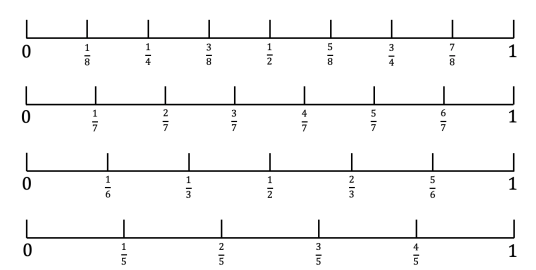
\includegraphics[width=0.75\linewidth]{Images/candidr.png}
        \caption{The set of candidates for $\frac{j}{r}$ in the $N = 8$ case}
        \label{fig:candidr}
    \end{figure}

    Note that some values (like those with denominators $2$, $3$, and $4$) are already covered by cases where $r = 6$ or $8$, due to reduced fraction equivalences. Figure~\ref{fig:combinedr} shows these candidates combined along a single axis for clarity.

    \begin{figure}[ht]
        \centering
        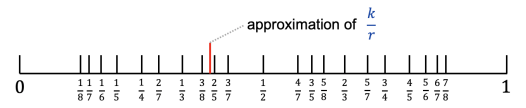
\includegraphics[width=0.75\linewidth]{Images/combinedr.png}
        \caption{Combined view of all candidate values of $\frac{j}{r}$ for $N = 8$}
        \label{fig:combinedr}
    \end{figure}

    Now suppose we obtain a $7$-bit approximation (i.e., $m = 7$) to one of these candidates. Say it's $0.0110011$. This binary value is exactly $\frac{51}{128}$, which is not one of the candidate values. However, the rational number $\frac{2}{5}$ is the unique candidate within a distance of $\frac{1}{2^7}$ from $0.0110011$.
\end{example}

In general, how precise must our approximation be to uniquely identify a single $\frac{j}{r}$? The answer depends on the smallest gap between any two distinct candidate values. This gap is smallest at the rightmost end of the spectrum: $\frac{1}{N - 1} - \frac{1}{N} \approx \frac{1}{N^2}$. To resolve such a gap, we must ensure
\[
2^m \approx N^2 \quad \Rightarrow \quad m \approx 2n,
\]
where $N$ is an $n$-bit number. Thus, choosing $m = 2n + 1$ ensures sufficient precision to isolate a unique rational value $\frac{j}{r}$ close to our measured approximation.

But perhaps you've already noticed a subtle issue: the problem of reduced fractions. Multiple distinct values of $j$ and $r$ can yield the same reduced fraction $\frac{j}{r}$. Therefore, although we may determine the correct reduced fraction from our approximation, we still need a method (e.g., post-processing or verification) to ensure we recover the actual order $r$ rather than a divisor of it.

Now, what do these reciprocals $\frac{1}{r}$ look like on the real line? Below is a visual representation of their positions for $r \in \{1,2,\ldots,N\}$.

\begin{figure}[ht]
    \centering
    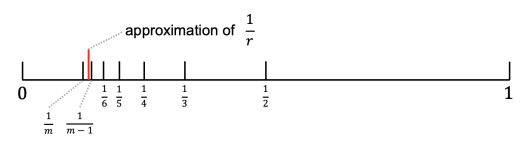
\includegraphics[width=0.75\linewidth]{Images/precisionr.png}
    \caption{The positions of $\left\{\frac{1}{1}, \frac{1}{2}, \ldots, \frac{1}{m}\right\}$ on the real line.}
    \label{fig:precr}
\end{figure}

The smallest gap occurs between $\frac{1}{N}$ and $\frac{1}{N-1}$. The size of this gap is
\[
\frac{1}{N-1} - \frac{1}{N} = \frac{N - (N-1)}{N(N-1)} = \frac{1}{N(N-1)} \approx \frac{1}{N^2}.
\]
This implies that our approximation must be within $\frac{1}{2N^2}$ of $\frac{1}{r}$ to distinguish $r$ correctly. Since $N$ is an $n$-bit number, $N \approx 2^n$, and thus
\[
\frac{1}{2N^2} \approx \frac{1}{2^{2n+1}},
\]
which corresponds to setting $m = 2n + 1$ bits of precision.

Another way to think about this is as follows. Our goal is to estimate $r$, given an approximation to $\frac{1}{r}$. Suppose that from the phase estimation procedure, we obtain some integer $j \in \{0, \ldots, 2^m - 1\}$ such that
\[
\frac{j}{2^m} \approx \frac{1}{r}.
\]
A natural strategy is to invert this approximation:
\[
\frac{1}{\frac{j}{2^m}} = \frac{2^m}{j}.
\]
This may not yield an integer since $\frac{j}{2^m}$ is only approximately equal to $\frac{1}{r}$. Therefore, we round to the nearest integer:
\[
r = \left\lfloor \frac{2^m}{j} + \frac{1}{2} \right\rfloor.
\]

However, this works only if the approximation is sufficiently accurate. Specifically, to ensure the correct rounding, we need
\[
\left| \frac{j}{2^m} - \frac{1}{r} \right| \leq \frac{1}{2r(r+1)}.
\]
This is because $\frac{1}{r}$ must be distinguishable from nearby values like $\frac{1}{r-1}$ and $\frac{1}{r+1}$, the closest other possible candidates. We don't know $r$, but we do know that $r < N$, so a sufficient condition is
\[
\left| \frac{j}{2^m} - \frac{1}{r} \right| \leq \frac{1}{2N^2}.
\]

Thus, we conclude that the number of bits of precision $m$ must satisfy $m \geq 2n + 1$ in order to determine $r$ reliably from the phase estimation outcome.

Indeed, this accuracy is sufficient. We can be sure that rounding $2^m / j$ to the nearest integer will yield $r$, provided that
\[
\left| \frac{2^m}{j} - r \right| < \frac{1}{2}.
\]
Assuming $|\epsilon| \leq \frac{1}{2N^2}$, where $\epsilon = \frac{j}{2^m} - \frac{1}{r}$, we have:
\begin{align*}
\left| \frac{2^m}{j} - r \right| &= \left| \frac{1}{\frac{1}{r} - \epsilon} - r \right| \\
&= \left| \frac{r^2 \epsilon}{1 - r\epsilon} \right| \\
&\leq \frac{\frac{r^2}{2N^2}}{1 - \frac{r}{2N^2}} = \frac{r^2}{2N^2 - r} \\
&\leq \frac{(N - 1)^2}{2N^2 - N} \leq \frac{1}{2}.
\end{align*}
Therefore, if we take $m = 2n$ in the phase estimation procedure, the resulting accuracy will be sufficient to recover $r$.

\vspace{0.5em}

But how do we find the rational number? If $N$ is an $n$-bit number, then the number of possible rational candidates $\frac{j}{r}$ is exponential in $n$, so a brute-force search is not feasible.

Fortunately, there is a known efficient algorithm that is tailor-made for this problem: the \textit{continued fractions algorithm}. This algorithm allows us to efficiently recover the pair $(j, r)$ from an $m$-bit approximation to $\frac{j}{r}$, provided the approximation is sufficiently close and $r < N$.

\subsection{The Continued Fractions Algorithm}

The reduction of order-finding to phase estimation is completed by describing how to obtain the desired answer $r$ from the result of the phase estimation algorithm, which outputs a real number $\phi \approx \frac{k}{r}$. We only know $\phi$ to $m = 2n + 1$ bits of precision, but we also know a priori that $\phi$ is close to a rational number whose denominator is bounded. If we can efficiently recover the nearest such rational approximation to $\phi$, we can obtain the value of $r$.

There is an algorithm that accomplishes this task efficiently, known as the \textit{continued fractions algorithm}. The following theorem explains why this algorithm satisfies our requirements:

\begin{theorem}
    Suppose $\frac{k}{r}$ is a rational number such that
    \[
    \left| \phi - \frac{k}{r} \right| \leq \frac{1}{2r^2}.
    \]
    Then $\frac{k}{r}$ is a convergent of the continued fraction expansion of $\phi$, and can be computed in $\mathcal{O}(n^3)$ time using the continued fractions algorithm.
\end{theorem}

The algorithm is based on the following well-known number-theoretic fact:

\textbf{Fact:}
    Given a real number $\alpha \in (0,1)$ and a bound $N \geq 2$, there exists at most one reduced fraction $\frac{x}{y}$ such that
    \[
    0 \leq x, y < N,\quad \gcd(x,y) = 1,\quad y \neq 0,\quad \text{and} \quad \left| \alpha - \frac{x}{y} \right| < \frac{1}{2N^2}.
    \]
    Moreover, given such an $\alpha$ and $N$, the continued fractions algorithm can find this $\frac{x}{y}$ (if it exists) using $\mathcal{O}((\log N)^3)$ bit operations.
    
Thus, once phase estimation yields a real number $\phi$ to sufficient precision (i.e., $m = 2n+1$ bits), we can recover the rational approximation $\frac{k}{r}$ using continued fractions, from which the order $r$ can be obtained.

\subsection{The Continued Fractions Algorithm}

The idea behind the continued fractions algorithm is to express real numbers using only integers, via expressions of the form
\[
[a_0, a_1, \ldots, a_M] = a_0 + \frac{1}{a_1 + \frac{1}{a_2 + \cdots + \frac{1}{a_M}}},
\]
where $a_0, a_1, \ldots, a_M$ are positive integers. (For applications in quantum computing, it is convenient to allow $a_0 = 0$ as well.) The $m$-th \textit{convergent} of this continued fraction (for $0 \leq m \leq M$) is the rational approximation $[a_0, \ldots, a_m]$.

The continued fractions algorithm is a method for computing the continued fraction expansion of any real number. It is best understood through an example. Suppose we want to decompose $\frac{31}{13}$ as a continued fraction. The steps are as follows:

\begin{enumerate}
    \item Split $\frac{31}{13}$ into its integer and fractional parts:
    \[
    \frac{31}{13} = 2 + \frac{5}{13}
    \]
    \item Invert the fractional part:
    \[
    \frac{31}{13} = 2 + \frac{1}{\frac{13}{5}}
    \]
    \item Apply the same steps to $\frac{13}{5}$:
    \[
    \frac{31}{13} = 2 + \frac{1}{2 + \frac{3}{5}} = 2 + \frac{1}{2 + \frac{1}{\frac{5}{3}}}
    \]
    \item Continue with $\frac{5}{3}$:
    \[
    \frac{31}{13} = 2 + \frac{1}{2 + \frac{1}{1 + \frac{2}{3}}} = 2 + \frac{1}{2 + \frac{1}{1 + \frac{1}{\frac{3}{2}}}}
    \]
    \item Finally, decompose $\frac{3}{2}$:
    \[
    \frac{3}{2} = 1 + \frac{1}{2}
    \]
\end{enumerate}

Thus, we obtain the full continued fraction representation:
\[
\frac{31}{13} = [2, 2, 1, 1, 2] = 2 + \frac{1}{2 + \frac{1}{1 + \frac{1}{1 + \frac{1}{2}}}}.
\]

It's clear that the continued fractions algorithm terminates after a finite number of \texttt{split} and \texttt{invert} steps for any rational number, since the numerators in the intermediate steps (31, 5, 3, 2, 1 in this example) strictly decrease.

\paragraph{Runtime Complexity.}  
How quickly does this termination occur? If $\frac{s}{r}$ is a rational number, and $s$ and $r$ are $n$-bit integers, then the continued fraction expansion can be computed using $\mathcal{O}(n^3)$ operations: $\mathcal{O}(n)$ split-and-invert steps, each requiring $\mathcal{O}(n^2)$ gates for basic arithmetic.

\paragraph{Application to Order Finding.}  
Since $\phi$ is an $m$-bit approximation of $k/r$ with $m = 2n+1$, we have
\[
\left| \phi - \frac{k}{r} \right| \leq 2^{-2n - 1}.
\]
Given that $r \leq N \leq 2^n$, this implies
\[
\left| \phi - \frac{k}{r} \right| \leq \frac{1}{2r^2},
\]
which satisfies the condition of the continued fractions theorem. Therefore, the algorithm can efficiently recover $\frac{k}{r}$ from $\phi$, and hence determine $r$.

\subsection{Post-processing via Continued Fractions}

Summarizing, given a phase estimate $\phi$, the continued fractions algorithm efficiently produces integers $s'$ and $r'$ with $\gcd(s', r') = 1$ such that
\[
\frac{s'}{r'} = \frac{s}{r},
\]
where $\frac{s}{r}$ is the true phase $\phi$ approximates. The value $r'$ is our candidate for the order. To verify whether $r'$ is the correct order, we compute
\[
a^{r'} \bmod N.
\]
If the result is $1$, then $r'$ is the order of $a$ modulo $N$, and we are done.

However, a subtle issue arises: multiple pairs $(k, r)$ can correspond to the same rational number. For instance, $\frac{34}{51} = \frac{2}{3}$. The continued fractions algorithm always returns the reduced form, so it is impossible to distinguish between $\frac{34}{51}$ and $\frac{2}{3}$ based solely on $\phi$. This means that we may recover a proper divisor of the actual order $r$. This issue disappears if $\gcd(k, r) = 1$, since the fraction $\frac{k}{r}$ is already in lowest terms in that case.

Recall that in our setting, $k$ is uniformly sampled from $\{0, 1, 2, \ldots, r - 1\}$. What is the probability that a randomly chosen $k$ is relatively prime to $r$? It is given by the ratio
\[
\frac{|\mathbb{Z}_r^*|}{|\mathbb{Z}_r|} = \frac{\phi(r)}{r},
\]
where $\phi(r)$ is Euler's totient function. While this ratio is not constant, it is known that
\[
\frac{\phi(r)}{r} = \Omega\left(\frac{1}{\log \log r}\right).
\]
For an $n$-bit modulus $r$, this is at least $\Omega\left(\frac{1}{\log n}\right)$. Hence, if we repeat the phase estimation procedure $\mathcal{O}(\log n)$ times, the probability that at least one of the resulting $k$ values is relatively prime to $r$ becomes constant. In the cases where $\gcd(k, r) > 1$, the continued fractions algorithm yields a denominator that is a proper divisor of $r$. This can be detected efficiently, since $a^{r'} \not\equiv 1 \pmod{N}$ in such cases.

\paragraph{Improved Strategy with Two Estimates.}

We can improve upon this strategy. Suppose we perform two independent repetitions of the phase estimation algorithm. Then we obtain two estimates $\frac{k_1}{r}$ and $\frac{k_2}{r}$ (where $r$ is unknown), and the continued fractions algorithm yields reduced forms
\[
\frac{k_1'}{r_1'} \quad \text{and} \quad \frac{k_2'}{r_2'},
\]
where $r_1'$ and $r_2'$ are divisors of $r$. It turns out that, with constant probability, the least common multiple satisfies
\[
\mathrm{lcm}(r_1', r_2') = r.
\]
Therefore, with just two independent runs of the phase estimation procedure—each using an independent eigenvector—the true order $r$ can be determined with constant probability (independent of $n$). This gives us an efficient and robust approach to quantum order finding.

The accuracy parameter $m$ is set to $2n$. The output of the measurement is then post-processed using the classical continued fractions algorithm, which yields a numerator $k$ and a denominator $r$. After two independent runs, we take the least common multiple of the two resulting denominators to obtain the order $r$ with constant probability. This success probability depends on both the correctness of the phase estimation output and the likelihood that the continued fractions algorithm yields the correct denominator. The total quantum gate complexity is $\mathcal{O}(n^2 \log n)$.

\begin{example}
    In the order-finding algorithm, the quantum state just before the inverse quantum Fourier transform is
    \[
    \ket{\psi} = \sum_{j=0}^{2^t-1} \ket{j} U^j \ket{1} = \sum_{j=0}^{2^t-1} \ket{j} \ket{x^j \bmod N},
    \]
    where the second register is initialized to $\ket{1}$. Show that the same state is obtained if we replace $U^j$ with a different unitary transform $V$ that acts as
    \[
    V \ket{j}\ket{k} = \ket{j} \ket{k + x^j \bmod N},
    \]
    and initialize the second register to $\ket{0}$. Also, describe how to construct $V$ using $\mathcal{O}(n^3)$ gates.

    \paragraph{Solution.}
    If the second register is initialized to $\ket{0}$, then applying $V$ yields:
    \[
    \ket{\psi} = \sum_{j=0}^{2^t-1} V \ket{j} \ket{0} = \sum_{j=0}^{2^t-1} \ket{j} \ket{x^j \bmod N},
    \]
    which is the same state as before. Hence, $V$ and $U^j$ produce the same result when applied appropriately.

    \paragraph{Gate Complexity of $V$.}
    Note that $x^j \bmod N$ can be computed via repeated modular multiplications. Decompose the exponent $j$ in binary:
    \[
    x^j \bmod N = x^{j_0 2^0} \cdot x^{j_1 2^1} \cdots x^{j_{t-1} 2^{t-1}} \bmod N,
    \]
    where each $j_k \in \{0, 1\}$ corresponds to a controlled modular multiplication by $x^{2^k} \bmod N$.

    Each modular multiplication can be performed using $\mathcal{O}(n^2)$ gates, and we require $t = \mathcal{O}(n)$ such multiplications (since $j$ ranges up to $2^t$), giving a total cost of $\mathcal{O}(n^3)$ gates for constructing $x^j \bmod N$.

    The final step is to add $k$ to the computed value, i.e., perform
    \[
    \ket{j} \ket{0} \mapsto \ket{j} \ket{x^j \bmod N},
    \]
    which involves an addition requiring $\mathcal{O}(n)$ gates. Therefore, the total complexity of implementing $V$ is still $\mathcal{O}(n^3)$ gates.
\end{example}

\begin{example}
    Show that the least common multiple of positive integers $x$ and $y$ is given by
    \[
    \operatorname{lcm}(x, y) = \frac{xy}{\gcd(x, y)},
    \]
    and that it can be computed in $\mathcal{O}(L^2)$ operations when $x$ and $y$ are $L$-bit integers.

    \paragraph{Proof.} 
    The least common multiple (LCM) of two positive integers $x$ and $y$ is the smallest positive integer that is a multiple of both. The greatest common divisor (GCD) of $x$ and $y$ is the largest positive integer dividing both $x$ and $y$.

    Let $m = \operatorname{lcm}(x, y)$ and let $M$ be any common multiple of $x$ and $y$. Then we can write:
    \[
    M = mq + r, \quad \text{for integers } q \text{ and } 0 \le r < m.
    \]
    Since both $x$ and $y$ divide $M$ and $m$, they also divide $r = M - mq$, implying $r$ is a common multiple of $x$ and $y$. But $m$ is the smallest such number, so we must have $r = 0$, i.e., $m \mid M$.

    Now let $d = \gcd(x, y)$. Then we can write:
    \[
    x = d \cdot x_1, \quad y = d \cdot y_1,
    \]
    where $\gcd(x_1, y_1) = 1$. Then,
    \[
    \operatorname{lcm}(x, y) = \operatorname{lcm}(d x_1, d y_1).
    \]
    Note that $d x_1 y_1$ is a common multiple of $x$ and $y$. Since $x$ and $y$ divide $d x_1 y_1$, it follows that:
    \[
    \operatorname{lcm}(x, y) \le d x_1 y_1 = \frac{xy}{\gcd(x, y)}.
    \]
    Conversely, suppose $\operatorname{lcm}(x, y) = m$. Then, since both $x$ and $y$ divide $m$, we can write:
    \[
    m = d x_1 y_1 q \quad \text{for some } q \in \mathbb{Z}.
    \]
    But then $q$ divides both $x_1$ and $y_1$, which are coprime, so $q = 1$. Thus,
    \[
    \operatorname{lcm}(x, y) = d x_1 y_1 = \frac{xy}{\gcd(x, y)}.
    \]

    \paragraph{Computational Complexity.} 
    The GCD can be computed using Stein's algorithm (binary GCD algorithm), which runs in $\mathcal{O}(L^2)$ bit operations for $L$-bit integers. Once the GCD is known, computing the LCM involves a multiplication and a division of $L$-bit numbers, both of which also require $\mathcal{O}(L^2)$ operations. Hence, the entire LCM computation takes $\mathcal{O}(L^2)$ operations.
\end{example}


\section{Performance}

How can the order-finding algorithm fail? There are two primary failure modes:

\begin{enumerate}
    \item The phase estimation algorithm might produce a poor approximation of $s/r$. However, this occurs with probability at most $\epsilon$, and the error can be made arbitrarily small by slightly increasing the number of qubits in the first register. This form of failure is negligible.

    \item A more serious issue arises when $s$ and $r$ share a common factor. In this case, the rational number $r'$ returned by the continued fractions algorithm might be a proper divisor of $r$, rather than $r$ itself.
\end{enumerate}

Fortunately, there are three standard strategies to circumvent this second issue:

\subsection{Method 1: Repeating with Random $s$ Until Coprime with $r$}

The most straightforward solution is to repeat the phase estimation procedure several times. For a randomly chosen $s \in \{1, \ldots, r-1\}$, the probability that $\gcd(s, r) = 1$ is $\phi(r)/r$, where $\phi$ is Euler's totient function. A well-known number-theoretic result shows that
\[
\frac{\phi(r)}{r} > \frac{1}{2 \log r},
\]
and since $r \leq N$, we also have $\frac{1}{2\log r} \geq \frac{1}{2 \log N}$. Thus, by repeating the algorithm $2 \log N$ times, we will—*with high probability*—observe a phase $s/r$ where $s$ is coprime to $r$, and hence the continued fractions algorithm will correctly return $r$.

\subsection{Method 2: Recursive Order Reduction}

Suppose the continued fractions algorithm gives us $r' < r$ due to $\gcd(s, r) > 1$. Since $s/r$ reduces to lowest terms, $r'$ must be a divisor of $r$ (unless $s = 0$, which occurs with probability at most $1/r \leq 1/2$). We can use this fact recursively:

\begin{enumerate}
    \item Replace $a$ with $a' \equiv a^{r'} \pmod{N}$.
    \item Compute the order of $a'$ using the same algorithm.
    \item If the returned order is $r''$, set $a'' \equiv (a')^{r''} \pmod{N}$.
    \item Repeat until the total accumulated product $r' \cdot r'' \cdot \ldots$ equals $r$.
\end{enumerate}

Each iteration reduces the current order by a factor of at least 2, so this method converges in at most $\log r = \mathcal{O}(n)$ iterations.

\subsection{Method 3: Using Least Common Multiple of Multiple Runs}

A better approach—requiring only a constant number of trials—is to repeat the phase estimation procedure twice. Suppose we obtain rational approximations $s_1/r_1$ and $s_2/r_2$ from two runs, and let $s_1$ and $s_2$ be their numerators. If $\gcd(s_1, s_2) = 1$, then we can recover $r$ by computing
\[
r = \operatorname{lcm}(r_1, r_2) = \frac{r_1 r_2}{\gcd(r_1, r_2)}.
\]

The probability that two random integers $s_1$ and $s_2$ are coprime is known to be at least:
\[
\Pr[\gcd(s_1, s_2) = 1] = \prod_q \left(1 - \frac{1}{q^2}\right) \geq \frac{1}{\zeta(2)} = \frac{6}{\pi^2} > \frac{1}{2},
\]
but for a simple bounding argument, we can write:
\[
1 - \sum_q \frac{1}{q^2} \geq 1 - \frac{3}{4} = \frac{1}{4}.
\]
So the probability of success in two trials is at least $1/4$.

\begin{example}
    Show that the least common multiple of positive integers $x$ and $y$ is
    \[
    \operatorname{lcm}(x, y) = \frac{xy}{\gcd(x, y)},
    \]
    and that this can be computed in $\mathcal{O}(n^2)$ bit operations when $x$ and $y$ are $n$-bit numbers.

    \textbf{Proof.} Write $x = d x_1$, $y = d y_1$ where $d = \gcd(x, y)$ and $\gcd(x_1, y_1) = 1$. Then any common multiple of $x$ and $y$ is a multiple of $d x_1 y_1$. Thus:
    \[
    \operatorname{lcm}(x, y) = d x_1 y_1 = \frac{xy}{\gcd(x, y)}.
    \]
    Using Stein’s binary GCD algorithm and standard long multiplication/division, this can be done in $\mathcal{O}(n^2)$ time.
\end{example}

\begin{example}
    For all $x \geq 2$, prove that:
    \[
    \int_x^{x+1} \frac{1}{y^2} \, dy \geq \frac{2}{3x^2}.
    \]
    Use this to show that:
    \[
    \sum_{q=2}^{\infty} \frac{1}{q^2} \leq \frac{3}{2} \int_2^{\infty} \frac{1}{y^2} \, dy = \frac{3}{4}.
    \]

    \textbf{Proof.} For $x \geq 2$,
    \[
    \int_x^{x+1} \frac{1}{y^2} \, dy = \left[ -\frac{1}{y} \right]_x^{x+1} = \frac{1}{x} - \frac{1}{x+1} = \frac{1}{x(x+1)} \geq \frac{2}{3x^2},
    \]
    since $x+1 \leq \frac{3}{2}x$ for $x \geq 2$.

    For bounding the sum:
    \[
    \sum_{q=2}^{\infty} \frac{1}{q^2} \leq \sum_{q=2}^{\infty} \frac{3}{2} \int_q^{q+1} \frac{1}{y^2} \, dy = \frac{3}{2} \int_2^{\infty} \frac{1}{y^2} \, dy = \frac{3}{2} \cdot \frac{1}{2} = \frac{3}{4}.
    \]
\end{example}

So, by setting $m = 2n$, applying the phase estimation algorithm, and then applying the continued fractions algorithm to the result, we can recover integers $x$ and $y$ such that
\[
\frac{x}{y} = \frac{k}{r}
\]
in lowest terms. This procedure may fail to find the exact value of $r$ if $\gcd(k, r) > 1$, but in that case we know that $y$ divides $r$. Thus, repeating the procedure multiple times (each time with a different random $k$) and computing the least common multiple of the resulting $y$ values gives $r$ with high probability.

\medskip

In summary, the complete order-finding algorithm proceeds as follows:

\begin{enumerate}
    \item Set $m = 2n$, where $n = \lfloor \log N \rfloor + 1$.
    
    \item Run the phase estimation circuit (see Figure~\ref{fig:orderfinding}) with the controlled-$U_{a,N}$ operator and the second register initialized to $\ket{1}$.
    
    \item Measure the first register to obtain a value $j$, which corresponds to the approximation $j/2^m \approx k/r$ for some integer $k$.
    
    \item Apply the continued fractions algorithm to the pair $(j, 2^m)$ with bound $N$ to obtain a candidate fraction $x/y \approx k/r$ in lowest terms.
    
    \item Repeat the above steps multiple times, collecting values $y_1, y_2, \ldots, y_t$ from each trial.
    
    \item Compute $\operatorname{lcm}(y_1, y_2, \ldots, y_t)$; with high probability, this equals $r$.
\end{enumerate}

This entire process is known as \textbf{Shor's algorithm for order finding}.

\medskip

To ensure that the estimate $j/2^m$ is sufficiently close to $k/r$ to be correctly identified by the continued fractions algorithm, we use $t$ ancilla qubits in the first register, where
\[
t = 2n + 1 + \left\lceil \log\left(2 + \frac{1}{2\epsilon} \right) \right\rceil.
\]
If we prepare the second register in the state $\ket{1}$ (which is trivial to construct), then for each $s \in \{0, 1, \ldots, r - 1\}$, we will obtain an estimate $\phi \approx s/r$ accurate to $2n + 1$ bits with probability at least $\frac{1 - \epsilon}{r}$.

\section{Complexity Analysis}

What resources does the quantum order-finding algorithm consume?

\begin{itemize}
    \item The Hadamard transform applied to $t = \mathcal{O}(n)$ qubits requires $\mathcal{O}(n)$ quantum gates.
    
    \item The inverse Quantum Fourier Transform (QFT) requires $\mathcal{O}(n^2)$ gates.
    
    \item The dominant cost in the quantum circuit comes from modular exponentiation, which can be implemented using repeated squaring and modular multiplication. This requires $\mathcal{O}(n^3)$ gates.
    
    \item After measuring the phase estimate, the continued fractions algorithm runs classically in $\mathcal{O}(n^3)$ time.
\end{itemize}

Thus, the total resource requirement to obtain a single candidate $r'$ is $\mathcal{O}(n^3)$. Using the third method (based on least common multiples) to recover the actual order $r$ from $r'$ requires only a constant number of repetitions. Hence, the total complexity of the algorithm remains:

\[
\mathcal{O}(n^3)
\]

and the algorithm succeeds with constant probability, independent of $n$.

The following summarizes the quantum order-finding algorithm:

\begin{algorithm}[H]
    \caption{Quantum Order-Finding Algorithm}
    \begin{algorithmic}[1]
        \State \textbf{Input:} A unitary black-box $U_{x,N}$ that performs the transformation:
        \[
        \ket{j}\ket{k} \mapsto \ket{j}\ket{x^j k \bmod N},
        \]
        where $x$ is coprime to an $n$-bit number $N$.

        \Statex \hspace{1em} $t = 2n + 1 + \lceil \log(2 + 1/2\epsilon) \rceil$ qubits initialized to $\ket{0}$ (first register), and $n$ qubits initialized to $\ket{1}$ (second register).

        \State \textbf{Output:} The smallest positive integer $r$ such that $x^r \equiv 1 \pmod{N}$.

        \State \textbf{Runtime:} $\mathcal{O}(n^3)$ operations. Succeeds with probability $\Theta(1)$.

        \State \textbf{Procedure:}
        \State \hspace{1em} \textbf{Initialize:} $\ket{0}\ket{1}$
        \State \hspace{1em} Apply Hadamard on the first register:
        \[
        \ket{0}\ket{1} \rightarrow \frac{1}{\sqrt{2^t}} \sum_{j=0}^{2^t - 1} \ket{j} \ket{1}
        \]
        \State \hspace{1em} Apply modular exponentiation (controlled-$U_{x,N}$):
        \[
        \rightarrow \frac{1}{\sqrt{2^t}} \sum_{j=0}^{2^t - 1} \ket{j} \ket{x^j \bmod N}
        \]
        \Statex \hspace{1em} This state is approximately:
        \[
        \approx \frac{1}{\sqrt{r 2^t}} \sum_{s=0}^{r-1} \sum_{j=0}^{2^t - 1} e^{2\pi i s j / r} \ket{j} \ket{u_s}
        \]
        \State \hspace{1em} Apply inverse QFT to the first register:
        \[
        \rightarrow \frac{1}{\sqrt{r}} \sum_{s=0}^{r - 1} \ket{\widetilde{s/r}} \ket{u_s}
        \]
        \State \hspace{1em} Measure the first register $\Rightarrow$ observe $\widetilde{s/r}$.
        \State \hspace{1em} Apply the continued fractions algorithm to estimate $r$.
    \end{algorithmic}
\end{algorithm}

\section{Summary}



\chapterreferences
